\subsection*{Change Help Pictures}
%motivation
Piktotegner has grown to be an application with numerous features for creating pictograms.
As of such, due to the scale of the application, people may be confused when using the application the first time.
The help pictures comes as a possible solution to this, where the user can open the help menu and look at help pictures to get a better understanding of how the application works.
Help pictures already exists from last semester, but has become outdated due to UI changes, which is also a reason for the creation of new help pictures to replace the old ones.

The help pictures are structured as a mini sequence, such that each help picture contains two images, aligned top and bottom.
The top image shows where to press to perform some action and the bottom image shows the result of performing that action.
In total, 24 new help pictures has been made and to view them you browse through them with a left and right arrow button.
An example of such a help picture can be seen in \figref{fig:helpCamera}.

\begin{figure}[h]
     \centering
     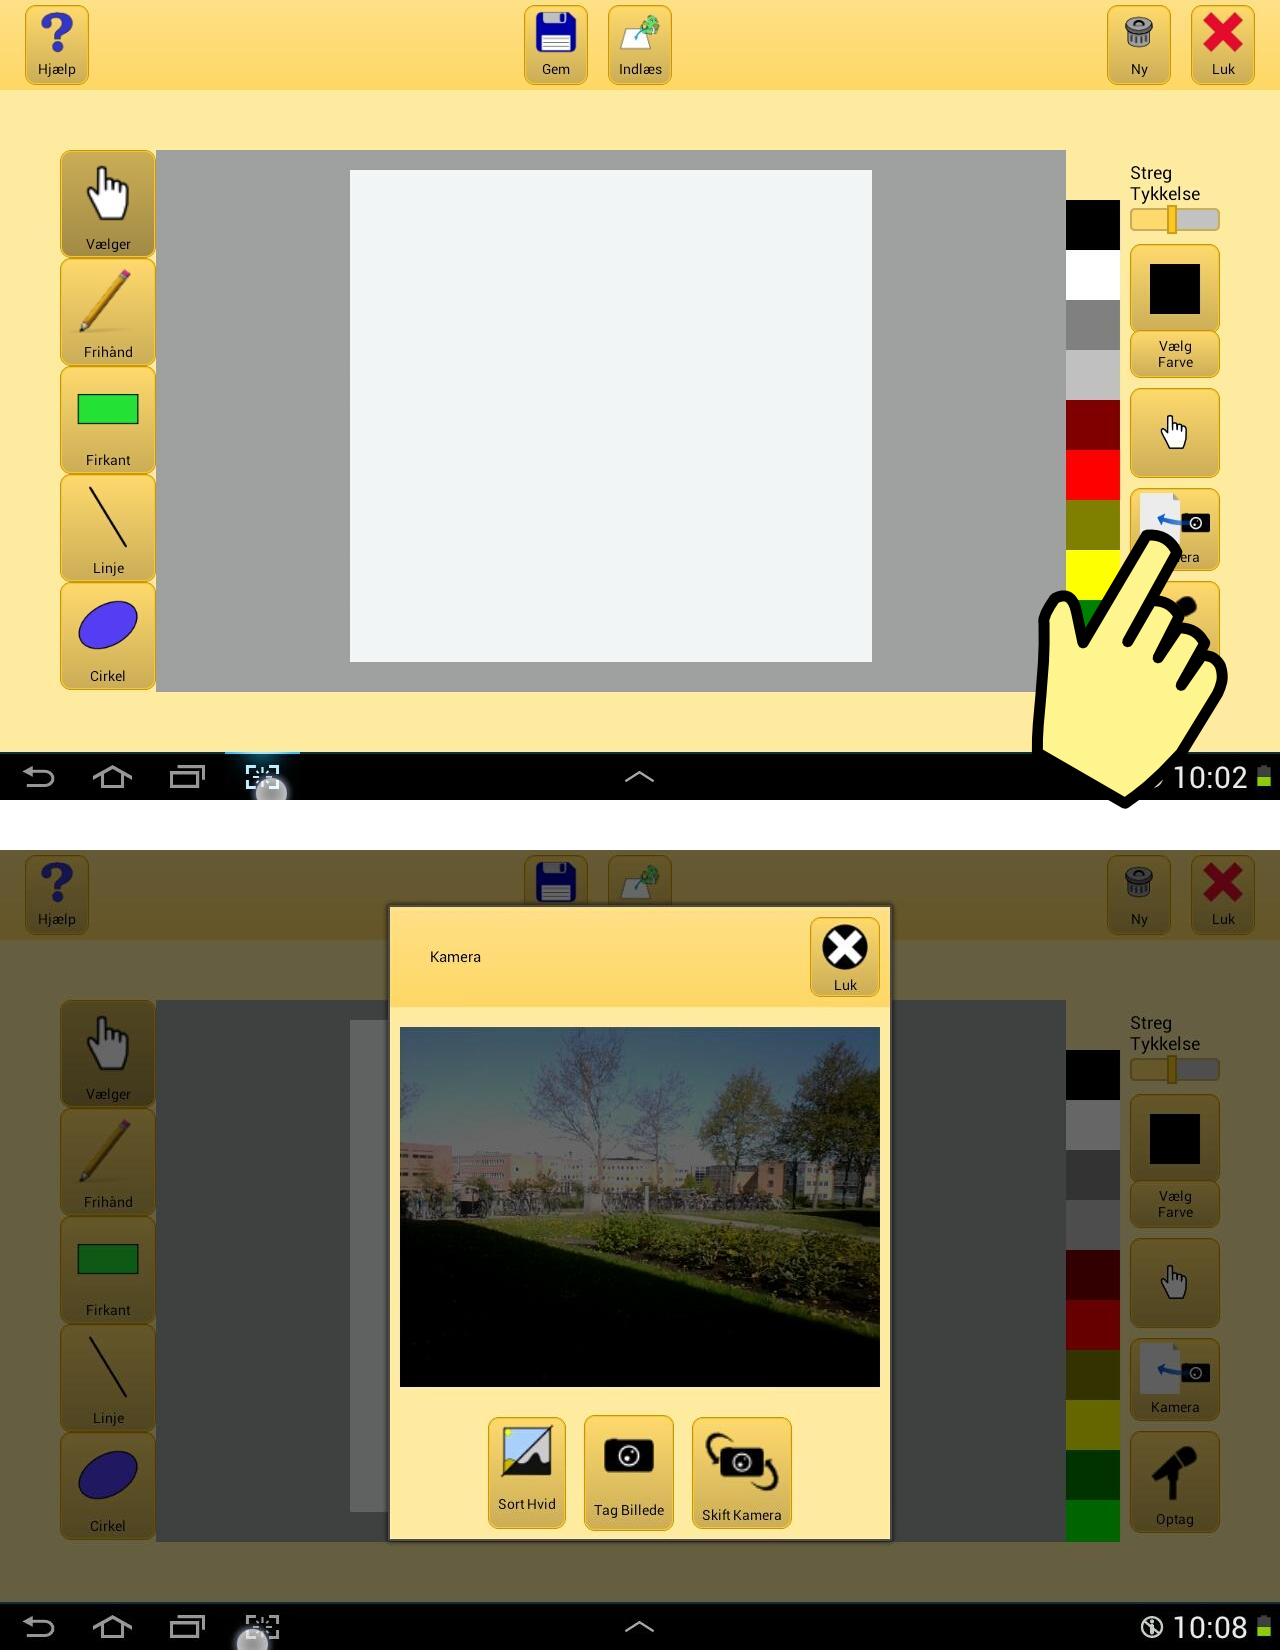
\includegraphics[scale=0.25]{sprint4/help_camera_1}
     \caption{Help picture for opening camera dialogue.}
     \label{fig:helpCamera}
\end{figure}

%How are the pictures structured

% further improvements?